% !TeX encoding = UTF-8
% !TeX spellcheck = en_GB
% !TeX program = xelatex

\documentclass[10pt, compress]{beamer}

\usetheme[usetitleprogressbar]{m}
%\usetheme{Boadilla}
\setbeamercovered{transparent}
%\useinnertheme{circles}
\setbeamertemplate{itemize items}[circle]

\title{Practical issues related to research/publication workflow}
\author{Lars Relund Nielsen}
\date{\today}
\institute{Department of Economics and Business}


% outline frame after each section
\AtBeginSection[]
{
   \begin{frame}
       \frametitle{Agenda}
       \tableofcontents[currentsection]
   \end{frame}
}
%\IfFileExists{upquote.sty}{\usepackage{upquote}}{}


%% --------------------------------------------------------------------------------------
%% Biblography
%% --------------------------------------------------------------------------------------

\usepackage[backend=bibtex, style=verbose-ibid]{biblatex}   
\addbibresource{litt.bib}

% 
\DeclareTextCommandDefault{\nobreakspace}{\leavevmode\nobreak\ } 


%% --------------------------------------------------------------------------------------
%% Quatation environment
%% --------------------------------------------------------------------------------------
\usepackage{tikz}
\usepackage{etoolbox}
%\usepackage{libertine} 
\newcommand*\quotefont{\fontfamily{LinuxLibertineT-LF}} % selects Libertine as the quote font
%\usepackage{newtxtext,newtxmath}
\newcommand*\quotesize{60} % if quote size changes, need a way to make shifts relative
% Make commands for the quotes
\newcommand*{\openquote}
   {\tikz[remember picture,overlay,xshift=-4ex,yshift=-2.5ex]
   \node (OQ) {\quotefont\fontsize{\quotesize}{\quotesize}\selectfont``};\kern0pt}
\newcommand*{\closequote}[1]
  {\tikz[remember picture,overlay,xshift=4ex,yshift={#1}]
   \node (CQ) {\quotefont\fontsize{\quotesize}{\quotesize}\selectfont''};}
\newcommand*\shadedauthorformat{\emph} % define format for the author argument
% Now a command to allow left, right and centre alignment of the author
\newcommand*\authoralign[1]{%
  \if#1l
    \def\authorfill{}\def\quotefill{\hfill}
  \else
    \if#1r
      \def\authorfill{\hfill}\def\quotefill{}
    \else
      \if#1c
        \gdef\authorfill{\hfill}\def\quotefill{\hfill}
      \else\typeout{Invalid option}
      \fi
    \fi
  \fi}
% wrap everything in its own environment which takes one argument (author) and one optional argument
% specifying the alignment [l, r or c]
\newenvironment{bigquote}[2][l]%
{\authoralign{#1}
\ifblank{#2}
   {\def\shadequoteauthor{}\def\yshift{-2ex}\def\quotefill{\hfill}}
   {\def\shadequoteauthor{\par\authorfill\shadedauthorformat{#2}}\def\yshift{-4ex}}
\begin{quote}\openquote}
{\shadequoteauthor\quotefill\closequote{\yshift}\end{quote}}
% now use 
% \begin{bigquote}[<alignment (l|r|c)>]{<author>}
%    text of quote
% \end{bigquote}
%% --------------------------------------------------------------------------------------

\begin{document}

%% ---------------------------------------------------------------------
\maketitle
%% ---------------------------------------------------------------------


%\section{Reproducible Research}

%% ---------------------------------------------------------------------
\begin{frame}{Reproducible Research}

\begin{bigquote}[r]{D. Donoho}
An article about computational science in a scientific publication is not the scholarship itself, it is merely advertising of the scholarship. The actual scholarship is the complete software development environment and the complete set of instructions which generated the figures.
\end{bigquote}

\end{frame}
% ---------------------------------------------------------------------


%% ---------------------------------------------------------------------
\begin{frame}{Reproducible Research}
\begin{itemize}[<+->]
\item Reproducible results: The verification of a scientific experiment by
  other researchers using an independent experiment.
\item Reproducible research idea: The ultimate
  product of academic research is the paper along with the full
  computational environment used to produce the results in the paper
  such as the code, data, etc. that can be used to reproduce the results
  and create new work based on the research.
\item Reproducible research = automation (by running a script everything should be done).
\end{itemize}

\end{frame}
%% ---------------------------------------------------------------------


%% ---------------------------------------------------------------------
\begin{frame}{Reproducible Research diagram}
\begin{figure}
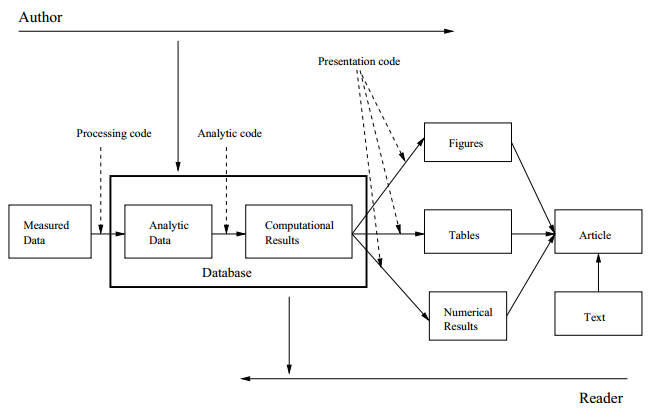
\includegraphics[width=0.8\linewidth]{graphic/distrib_research_diagram}
\caption{The research pipeline as a model for reproducible research \cite{Peng09}.}
\end{figure}


\end{frame}
%% ---------------------------------------------------------------------


%% ---------------------------------------------------------------------
\begin{frame}{Why Reproducible Research}

\begin{itemize}[<+->]
\item Automatically regenerate documents when code, data, or assumptions change (good after receiving a review).
\item Eliminate errors that occur when copy/transfer results into documents.
\item Preserve your own ``meta'' comments about why analysis was performed in a certain fashion.
\item Documentation for the analytic and computational processes from which
  conclusions are drawn (literal programming).
\item You may get a greater network and may be cited more.
\end{itemize}

\end{frame}
%% ---------------------------------------------------------------------



%% ---------------------------------------------------------------------
\begin{frame}{Tools for Reproducible Research}

\begin{itemize}[<+->]
\item R: Program computing and producing graphics (you may even use c or c++ for fast computations).
\item RStudio: Programming environment/editor for R
\item Using RStudio you can weave you computations together with your paper using knitr, LaTeX and R Markdown (can even make a Word file).
\item Git: A distributed revision control system.
\item Github: A web-based Git repository hosting service.
\end{itemize}

\end{frame}
%% ---------------------------------------------------------------------



%% ---------------------------------------------------------------------
\begin{frame}{How to do reproducible Research in OR}

\begin{itemize}[<+->]
\item Automate your work flow. Create a script that run your code and embed the results in your paper. 
\item Use a revision control system when your write your code (this may even be useful when write your paper).
\item Create graphics automatically.
\item Use \href{http://en.wikipedia.org/wiki/Literate_programming}{literal programming} (\href{http://roxygen.org/}{Roxygen} or \href{http://www.doxygen.org/}{doxygen})
\item Make your code open source with easy access (e.g. using github or CoinOR)
\item Make your test instances public available.
\end{itemize}

\end{frame}
%% ---------------------------------------------------------------------



%% ---------------------------------------------------------------------
\begin{frame}{More information}

\begin{itemize}
\item \href{http://en.wikipedia.org/wiki/Reproducibility}{Wikipedia (web)}, \href{http://kbroman.org/knitr_knutshell/pages/reproducible.html}{Comments on reproducibility (web)}.
\item The paper by \citeauthor{Nestler11} related to OR\footcite{Nestler11}.
\item The paper by \citeauthor{Peng09}\footcite{Peng09}.
\item A paper by \citeauthor{Stodden13} comparing different journals policies about reproducible research\footcite{Stodden13}.
\item A paper about \href{http://www.coin-or.org/}{CoinOR}\footcite{Lougee-Heimer03}.
\end{itemize}

\end{frame}
%% ---------------------------------------------------------------------



\end{document}
